\section{Introduction}

\subsection{Curse of Dimensionality}

\begin{frame}{Curse of Dimensionality}
    \begin{itemize}
        \item Increasing dimension leads to increasing data space\\$\rightarrow$ Distance measures perform poorly
    \end{itemize}

    \begin{figure}
        \centering
        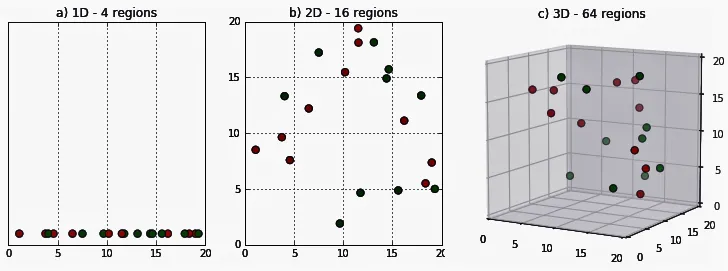
\includegraphics[width=0.9\linewidth]{img/dimension.png}
        \caption{Increase dimension $\to$ Sparse data $\to$ Poor measurement}
        \label{fig:enter-label}
    \end{figure}
\end{frame}

\begin{frame}{Curse of Dimensionality}
    \begin{columns}
        \begin{column}{0.6\textwidth}
            \begin{itemize}
                \item Increasing dimension leads to increasing data space\\$\rightarrow$ Predictive models become less effective at exploring patterns
            \end{itemize}
        \end{column}

        \begin{column}{0.5\textwidth}
            \begin{figure}
                \centering
                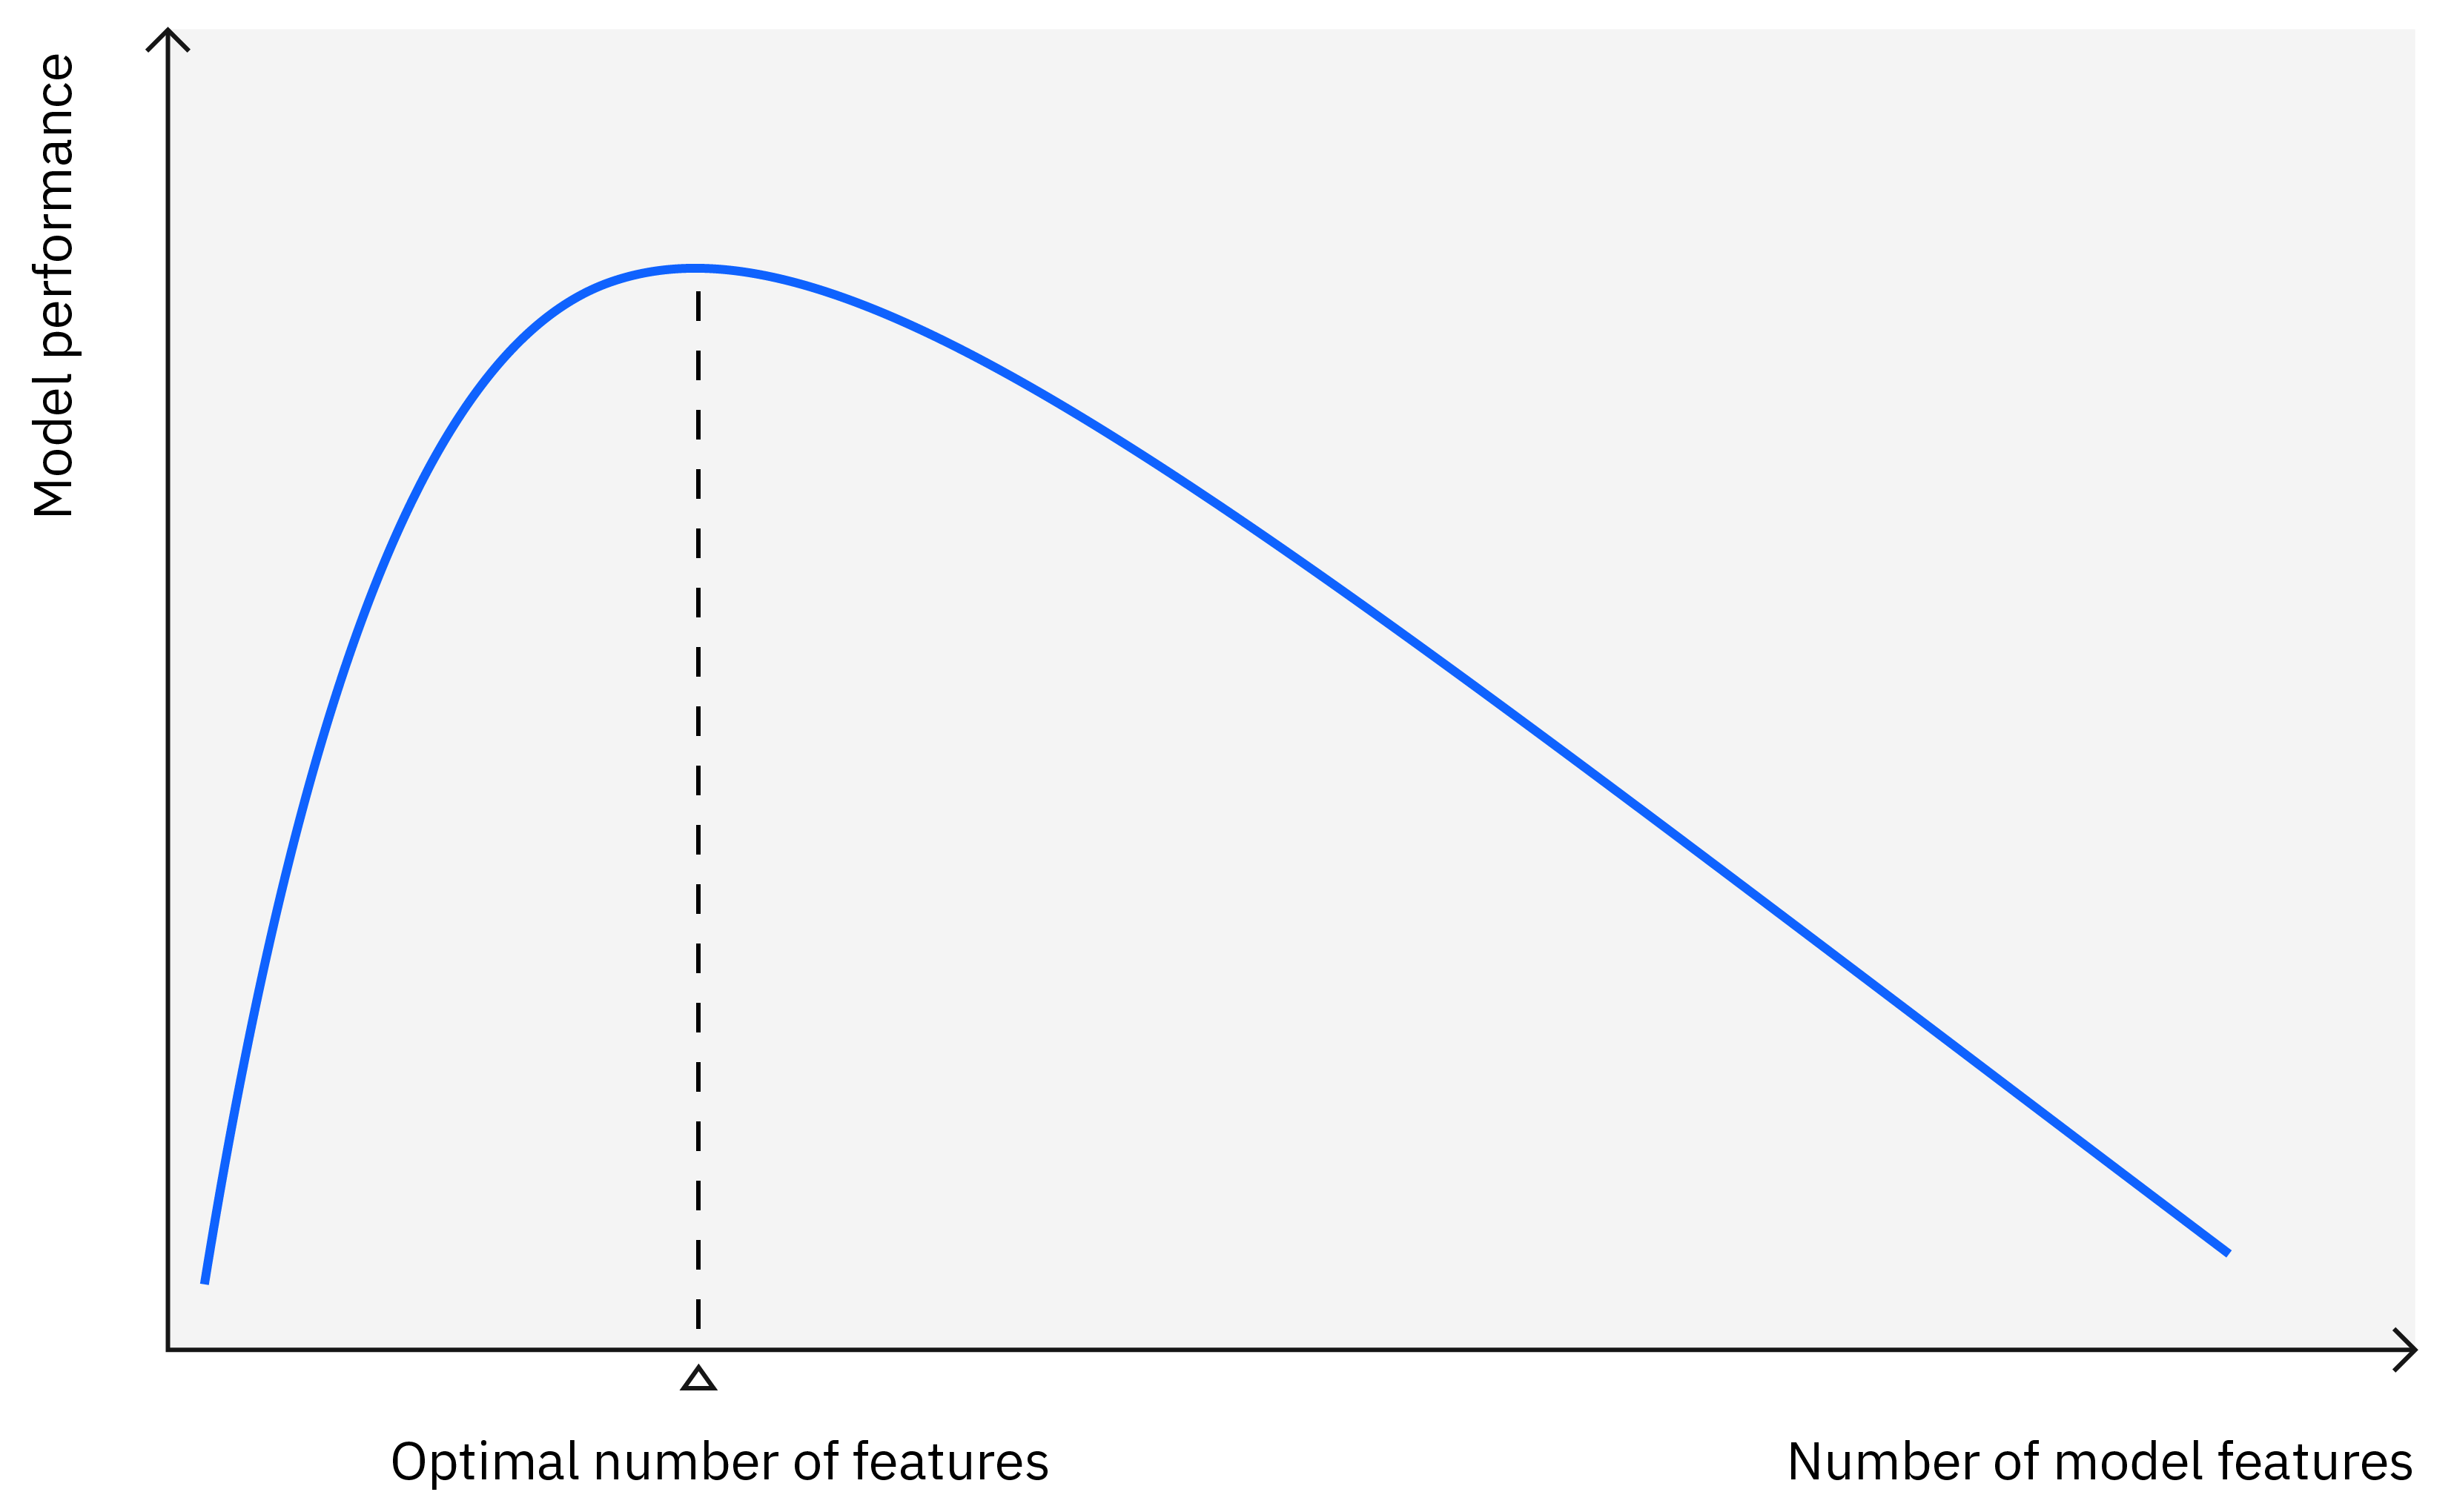
\includegraphics[width=\linewidth]{img/model_performance.png}
                \caption{Model performance vs. \#feature}
                \label{fig:enter-label}
            \end{figure}
        \end{column}
    \end{columns}
\end{frame}

\subsection{Dimensionality reduction}

\begin{frame}{Dimensionality reduction}
    \begin{columns}
        \begin{column}{0.6\textwidth}
            \begin{itemize}
                \item \textbf{Transform} $n$-dim data to $k$-dim data ($k<n$) while \textbf{preserving} as much information as possible
                \item In the example, we reduce datapoint from 2-D to 1-D (on x-axis)
            \end{itemize}
        \end{column}

        \begin{column}{0.5\textwidth}
            \begin{figure}
                \centering
                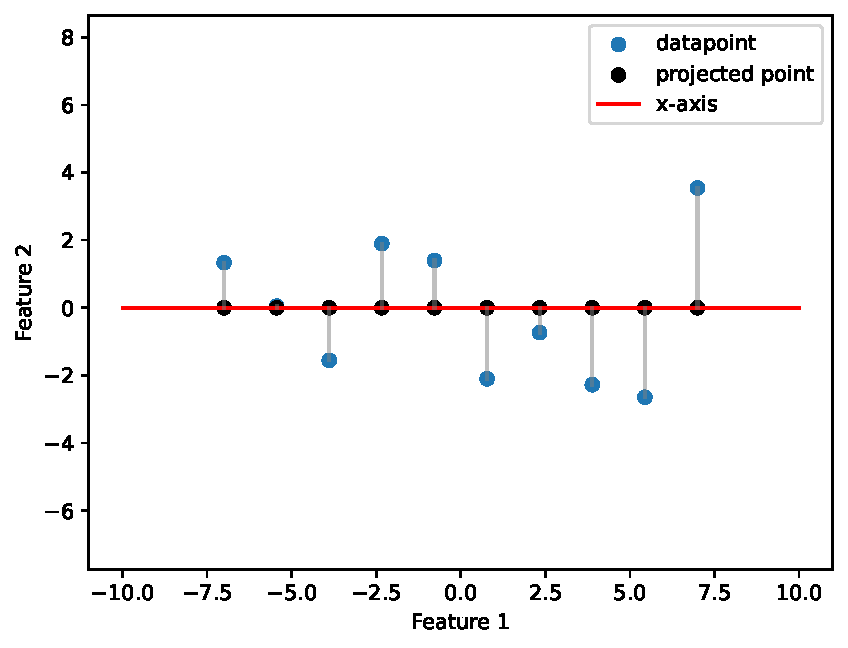
\includegraphics[width=\linewidth]{img/dp.pdf}
                \caption{Project data onto x-axis}
                \label{fig:enter-label}
            \end{figure}
        \end{column}
    \end{columns}
\end{frame}

\begin{frame}{Dimensionality reduction}
    \begin{columns}
        \begin{column}{0.6\textwidth}
            \begin{itemize}
                \item What if x-axis and y-axis are not enough to preserve information?\\$\rightarrow$ Project data onto a new axis
                \item Preserving information $\equiv$ \textbf{Maximizing standard deviation}\\$\rightarrow$ Idea of PCA
            \end{itemize}
        \end{column}

        \begin{column}{0.5\textwidth}
            \begin{figure}
                \centering
                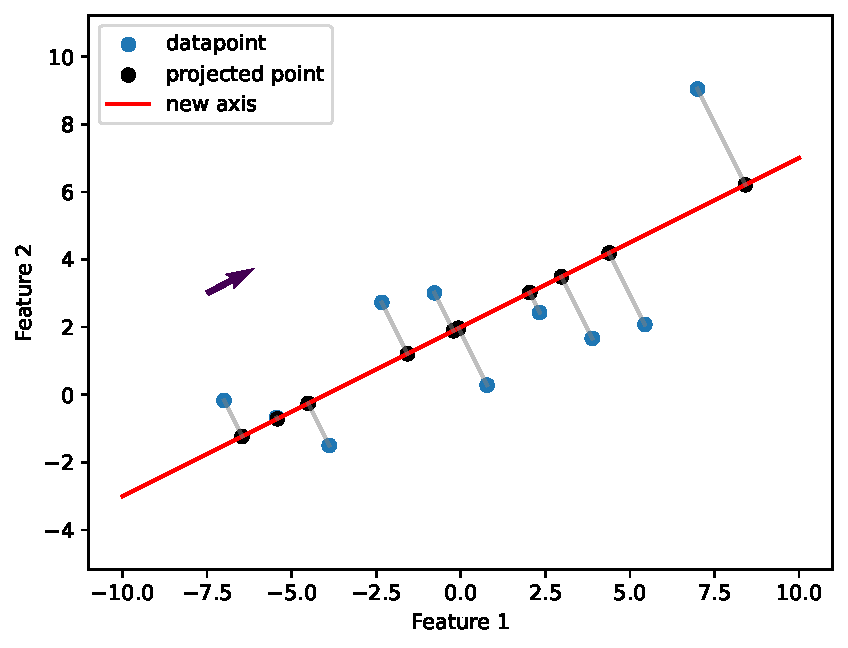
\includegraphics[width=\linewidth]{img/dp1.pdf}
                \caption{Project data onto a new axis}
                \label{fig:enter-label}
            \end{figure}
        \end{column}
    \end{columns}
\end{frame}
